\chapter{Marco Teórico Conceptual}


\section{Aprendiendo a partir de datos}
Existen varios acercamientos de aprendizaje máquina automático, pero uno de los acercamientos más exitosos ha sido el llamado aprendizaje basado en el gradiente. El modelo de aprendizaje calcula una función $Y^p=F\left(Z^p,W\right)$[3] donde $Z^p$ es la p-th patrón de entrada, $W$ representa la colección de parámetros ajustables en el sistema y  $Y^p$ puede ser interpretada como la etiqueta o clase del patrón $Z^p$, o la probabilidad asociada a cada clase a predecir. Es decir que a partir de una entrada se predice la clasificación deseada por medio de una función F.

$E^p=D\left(D^p,F\left(Z^p,W\right)\right)$ [3], es una función que mide la discrepancia o error entre $D^p$ el cuál es el valor correcto que deseamos predecir a partir del patrón de entrada $X^p$ y la predicción $Y^p$. Esto implica tener una base de datos con los patrones de entrada con su respectiva salida correcta para poder realizar esta operación con la cuál se entrena el modelo. Con el cálculo del error de cada predicción se puede calcular el promedio y obtener un error de entrenamiento $E_{train}\left(W\right)$ que se llamará función de costo o pérdida. Así muchos algoritmos de aprendizaje tratan de minimizar $E\left(W\right)$. 


\section{Gradiente descenciente}
El algoritmo de gradiente descendiente intenta minimizar la función de costo $E\left(W\right)$ a través de variaciones en los pesos $W$. Estas variaciones son introducidas a cada peso partir del gradiente de la función de perdida con respecto a los pesos. Pero para ello se tiene que cumplir que los parámetros de W son valores reales para los cual la función de costo es una función continua y diferenciable, de esta manera se introducen variaciones en cada parámetro de W iterativamente de la siguiente forma:
$W_k=W_{k-1}-\epsilon\frac{\partial E\left(W\right)}{\partial W}$[3]
Existen variaciones del gradiente descendiente siendo el presentado uno de los más simples.

\section{Perceptrón}
El perceptrón es un modelo computacional de una neurona[4], donde una sola neurona tiene varias entradas (dentritas), un cuerpo celular y una salida (axón). Replicando esto el perceptrón tiene varias entradas y una sola salida, el cuál consiste en un vector de “pesos” w = [w1 … wm], un peso para cada entrada más un “bias” o tendencia cuyo parámetro es descrito como b.
Con los parámetros dados w y b el perceptrón realiza el siguiente cálculo:
$$f\left(x\right)=1\ \ \ \ \ \ \ \ \ \ \ \ if\ b+\sum_{i=1}^{l}{x_iw_i}>0$$
$$f\left(x\right)=0\ \ \ \ \ \ \ \ \ \ \ \ \ \ \ de\ otra\ manera$$
Donde $f\left(x\right)$ se llama función de activación.
El algoritmo del perceptrón busca obtener o aprender los pesos w tales que dados los datos de cada ejemplo de entrenamiento $x^k=\left[x_1^k ... x_j^k\right]$, se obtenga la correcta clasificación binaria $a^k$, donde $a^k$ será 1 o 0 en este caso. 
\begin{figure}[htbp]
\begin{center}
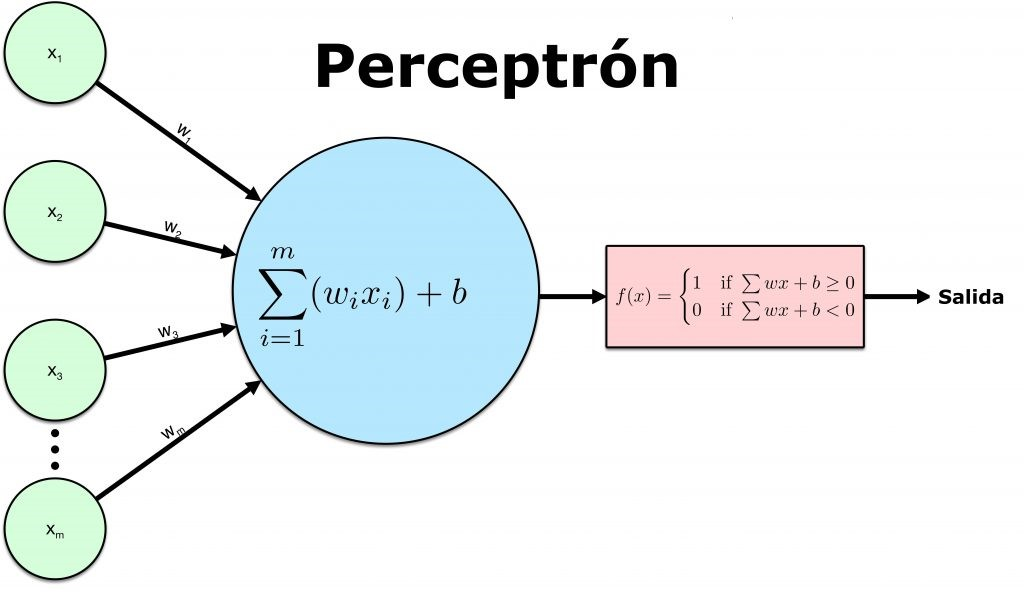
\includegraphics[width=3in]{capítulo3/Perceptron.jpg}
%http://blog.josemarianoalvarez.com/2018/06/10/el-perceptron-como-neurona-artificial/
\caption{Modelo del perceptrón}
\label{fig:perceptron}
\end{center}
\end{figure}
A continuación, se presenta el algoritmo del perceptrón[4]:
\begin{enumerate}
    \item Inicializar los parámetros w y b
    \item Durante N iteraciones (definidas por el desarrollador) o hasta que los pesos no cambien realizar lo siguiente:
    \begin{enumerate}
        \item Para cada ejemplo de entrenamiento $x^k$ con respuesta $a^k$
             \begin{itemize}
                 \item Calcular $f\left(x^k\right)$
                 \item Si $a^k\ -\ f\left(x^k\right)\ =\ 0$  continua
                 \item Si no, actualizar todos los pesos como a continuación $$ w_i = w_i+\left(a^k-f\left(x^k\right)\right)x_i $$
             \end{itemize}
    \end{enumerate}
\end{enumerate}
Donde si existe una configuración de pesos w con los cuales se puedan clasificar correctamente cada elemento de entrenamiento, el algoritmo lo encontrará, aunque en ejemplos reales no siempre es posible, el algoritmo puede encontrar una configuración de pesos w para clasificar correctamente un porcentaje de los elementos de entrenamiento.
En casos donde se necesite más clases se puede realizar incrementando la cantidad de perceptrones por cada clase, siendo el valor 0 el indicador de no pertenencia a la clase y el número 1 la pertenencia a la clase, teniendo así una llamada red neuronal.
\section{Red Neuronal Clásica}
Cómo se ha visto con el perceptrón, una red neuronal clásica consiste en conjunto de modelos computacionales llamadas neuronas, las cuales tienen parámetros ajustables w y “bias” que, por medio de un algoritmo, la red puede aprender a clasificar correctamente las clases a partir de los datos de entrada $x^k$.
\begin{figure}[htbp]
\begin{center}
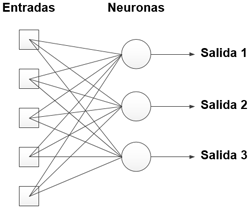
\includegraphics[width=3in]{capítulo3/RedNeuronalClasica.png}
%https://www.ediciones-eni.com/open/mediabook.aspx?idR=6d7e746f6a1fe07834a44f834c84d6ba
\caption{Modelo de una red neuronal de una sola capa}
\label{fig:rnc}
\end{center}
\end{figure}
En la Figura~\ref{fig:rnc} se puede observar un modelo de red neuronal, cuyas neuronas tienen una salida. Ahora, las salidas de las neuronas en la imagen podríamos tomarlas como entrada para un siguiente conjunto de neuronas, a cada conjunto de neuronas se les llama capas, siendo una capa las neuronas que reciben la entrada original, una segunda capa de neuronas como entrada la salida de la primera capa, teniendo una llamada red neuronal multicapa, donde a las capas entre la entrada y la salida se les llama capas ocultas como se presenta en la Figura~\ref{fig:rnc2}. 
De esta manera se pueden obtener redes neuronales de n capas, por lo que cada capa aumenta el tamaño o la “profundidad” de la red neuronal, y es aquí de donde procede el termino aprendizaje profundo o también conocido en inglés como “Deep learning”.
\begin{figure}[htbp]
\begin{center}
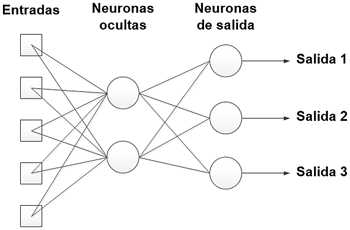
\includegraphics[width=3in]{capítulo3/RedNeuronalClasica2.png}
%https://www.ediciones-eni.com/open/mediabook.aspx?idR=dd1e7c64bbcc8628f67483605a21d1d2
\caption{Modelo de una red neuronal con una capa oculta}
\label{fig:rnc2}
\end{center}
\end{figure}
\section{Red Neuronal Feed Fordward y Back Propagation}
Son redes neuronales cuyo grafo con dirección no contienen ciclos, normalmente las redes neuronales multicapa utilizan un algoritmo de gradiente descendiente para calcular el valor de modificación de los pesos w, donde la diferencia de las neuronas del tipo perceptrón es el cambio de la función de activación, donde la función de activación del perceptrón está dada por:
$$f\left(\ x\right)=1\ \ \ \ \ \ \ \ \ \ \ \ if\ b+\sum_{i=1}^{l}{x_iw_i}>0$$
$$f\left(x\right)=0\ \ \ \ \ \ \ \ \ \ \ \ \ \ \ de\ otra\ manera$$
Esto debido que, para hacer uso del gradiente descendiente necesitamos que la función de costo o pérdida sea diferenciable y continua para el conjunto de valores reales de los pesos w. Dado que la función de pérdida $E^p=D\left(D^p,F\left(W,Z^p\right)\right)$[3] depende de la función de activación, la función del perceptrón no cumple los requisitos para implementar el gradiente descendiente.
Existen varias funciones de activación, una de las funciones usadas para las redes neuronales “feed forward” es la función sigmoide:
$$f\left(z\right)=\frac{1}{1+e^{-z}}$$
 La cual es derivable:
$$f^\prime\left(z\right)=f\left(z\right)\left(1-f\left(z\right)\right)$$
Donde 
$$z=\ b+\sum_{i=1}^{l}{x_iw_i}$$
Por lo cual se puede utilizar como función de activación y poder calcular el gradiente de la función de perdida para actualizar los pesos w. A dicho proceso con el cuál se calcula el gradiente a partir de la función de costo o pérdida y se actualizan los pesos w se le llama “back propagation”.

\section{Red Neuronal Convolucional}
Hasta ahora se ha considerado las redes neuronales completamente conectadas, pero estas también pueden ser parcialmente conectadas y un caso especial son las redes neuronales convolucionales, las cuales son muy recurridas es visión computacional.[4]
Las redes convolucionales combinan tres ideas para asegurar algún grado de invarianza en deslizamiento, escala y distorsión: campos receptivos locales, pesos compartidos y sub muestreo espacial o temporal. Los campos receptivos locales son llamados filtros o kernel, donde para una imagen en 2 dimensiones un filtro de dimensión 3x3, como ejemplo se podría ver de la siguiente forma:

$$\begin{matrix}a_1^1&a_1^2&a_1^3\\a_2^1&a_2^2&a_2^3\\a_3^1&a_3^2&a_3^3\\\end{matrix}$$

De una imagen de dimensión nxm se toma una parte de la dimensión del filtro viendo la parte superior izquierda como el punto de partida, y se realiza un producto punto, luego se toma de nuevo otra parte de la imagen de 3x3 pero esta vez tomamos los valores que están hacia la derecha desplazando la ventana un paso, uno en este caso y se realiza la misma operación con el filtro. Se repite la misma operación de desplazamiento y producto punto sobre toda la imagen, donde los valores resultantes dan otra imagen después de haber pasado por el filtro. Dicho filtro puede contener valores que “filtren” líneas verticales, horizontales, esquinas o puntos finales. Por lo que la imagen puede pasar por varios filtros obteniendo por cada filtro un mapa de característica y al final varios mapas con diferentes características. Esta capa de operaciones con filtros y desplazamiento se llama capa convolucional. Con este tipo de capa se busca que la red pueda aprender a partir de las características obtenidas por los filtros en lugar de los datos crudo de los pixeles.
Otra capa en una red convolucional es llamada “pooling” o de agrupación, que es un sub muestreo de la imagen de entrada para reducir sus dimensiones, la operación que realiza puede ser que a partir de una ventana por ejemplo de dimensión de 2x2 de la imagen de entrada y obtener el mayor valor que pasara a conformar la imagen reducida de salida, al finalizar el barrido sobre la imagen. Con este tipo de capa se busca reduciendo la sensibilidad de la red al desplazamiento y las distorsiones de la imagen entrada.
\begin{figure}[htbp]
\begin{center}
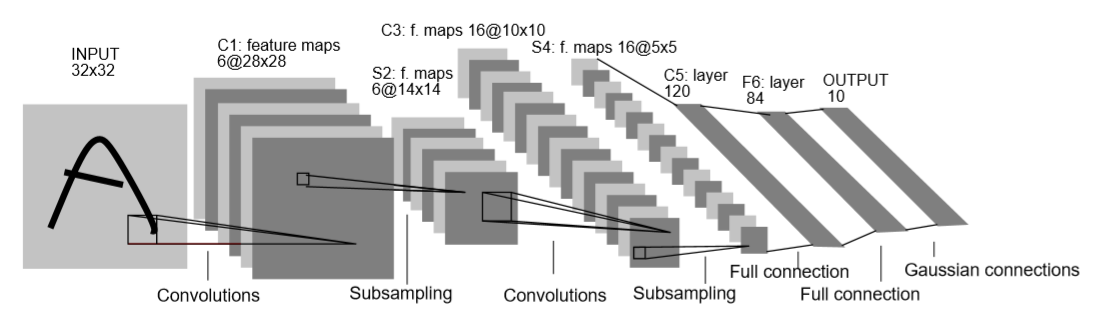
\includegraphics[width=4in]{capítulo3/LeNet.png}
%Y. LeCun, L. Bottou, Y. Bengio, y P. Haffner, «Gradient-Based Learning Applied to Doument Recognition», Proc. of the IEEE, November 18.
\caption{Modelo de una red neuronal con una capa oculta}
\label{fig:lenet}
\end{center}
\end{figure}
En la Figura~\ref{fig:lenet} se presenta un ejemplo de una red convolucional llamada LeNet-5 [3] en donde se puede observar 3 capas convolucionales C1, C3  y C5, dos capas de agrupación S2 y S4 y una capa completamente conectada.

%[1]	J. Schmidhuber, «Deep Learning in Neural Networks: An Overview», Neural Networks, vol. 61, pp. 85-117, ene. 2015, doi: 10.1016/j.neunet.2014.09.003.
%[2]	«ImageNet Large Scale Visual Recognition Competition (ILSVRC)». http://image-net.org/challenges/LSVRC/ (accedido oct. 07, 2019).
%[3]	Y. LeCun, L. Bottou, Y. Bengio, y P. Haffner, «Gradient-Based Learning Applied to Doument Recognition», Proc. of the IEEE, November 18.
%[4]	E. Charniak, Introduction to Deep Learning, 1st ed. The MIT Press, 2018.
%[5]	«Red neuronal artificial», Wikipedia, la enciclopedia libre. oct. 04, 2019, Accedido: oct. 06, 2019. [En línea]. Disponible en: https://es.wikipedia.org/w/index.php?title=Red_neuronal_artificial&oldid=119954405.
%[6]	V. E. Bondarenko, «Artificial neural networks», Salem Press Encyclopedia of Science. Salem Press, 2018.
%[7]	«t8neuronales.pdf». Accedido: oct. 06, 2019. [En línea]. Disponible en: http://www.sc.ehu.es/ccwbayes/docencia/mmcc/docs/t8neuronales.pdf.
%[8]	«Dialnet-ENTRENAMIENTODEUNAREDNEURONALARTIFICIALUSANDOELALG-4844874.pdf». .
%[9]	S. Shalev-Shwartz y S. Ben-David, Understanding Machine Learning from Theory to Algorithms. Cambridge University Press, 2015.
